%
%  愛知工業大学 情報科学部 情報科学科
%    要旨集用LaTeXテンプレート(2016.11.28)
%
%  original by Nobuhiro Ito
%  revised by Susumu Suzuki & Masashi Morimoto on 2016.11.28
%
\documentclass{jarticle}
\pagestyle{empty}

%% レイアウト
\setlength{\topmargin}{-10.4mm}
\setlength{\headheight}{0mm}
\setlength{\headsep}{0mm}
\setlength{\textheight}{262mm}
\setlength{\textwidth}{180mm}
%\setlength{\topskip}{7mm}
\setlength{\evensidemargin}{-10.4mm} 
\setlength{\oddsidemargin}{-10.4mm} 
\setlength{\columnsep}{8mm}

%% パッケージ環境
% graphicx: 画像読み込み
%  dvipdfmxをドライバ指定することでpdf/png/jpeg形式の図を利用可能
%  異なるドライバを利用する場合はそのドライバ指定に変更
% \usepackage{graphicx} % suzuki
\usepackage[dvipdfmx]{graphicx} % suzuki
% subcaption: subfigureを置き換えたパッケージ（複数の図用）
% \setlength{\footskip}{12mm}
% \usepackage{subfigure}	 % suzuki
\usepackage{subcaption} % suzuki
% color：文章に色をつけたいとき
%  利用例：\textcolor{red}{文章}
% \usepackage{color}
\usepackage{booktabs}
\usepackage{setspace}

% 行間調整
\setstretch{0.9}

%sectionのフォントサイズ修正
\makeatletter
\def\section{\@startsection {section}{1}{\z@}{2.5ex plus -1ex minus -.2ex}{1.3 ex plus .1ex}{\large\bf}}
\makeatother 

%subsectionのフォントサイズ修正
\makeatletter
\def\subsection{\@startsection {subsection}{1}{\z@}{1.5ex plus -1ex minus -.4ex}{0.3 ex plus .1ex}{\bf}}
\makeatother 

\begin{document}
\twocolumn[

    \begin{center}
        %タイトル
        {\LARGE \textbf{在室予測に基づく帰宅同行支援システムに関する研究}}\\
        %サブタイトル
        %{\Large \textbf{必要に応じてサブタイトル}}
    \end{center}

    \begin{center}
        % 著者
        \begin{tabular}{cccc}
            % 1名の場合
            \multicolumn{4}{c}{X22043 佐藤 綾花} \\
            % 2名の場合
            %& K11002 愛工七音 & X11003 愛工頼音 &\\
            % 3名の場合
            %K11001 愛工総和 & K11002 愛工今鹿 & X11003 愛工姫星&\\
            % 4名の場合
            % K11001 愛工総和 & K11002 愛工今鹿 & X11003 愛工姫星& X11004 愛工緑輝\\
            % 指導教員
            \multicolumn{4}{c}{\textbf{指導教員} 梶 克彦}
        \end{tabular}
        \hspace{2zw}
    \end{center}
]

%--------------------------------------------
\section{はじめに}
\label{sec:intro}
対面でのコミュニケーションは組織内の関係構築や業務効率において重要な役割をもつ．
リモートワークからハイブリッドワークに移行する傾向があり，オフィスに出社する機会が再び増加している．
これに伴い，対面機会を効果的に活用するためのコミュニケーション支援の重要性が高まっている．
%

こうした背景からコミュニケーションの支援を行う研究が進んでいる．例えば個別化が進むオフィスを対象としコミュニケーションのきっかけを提供するシステム\cite{ura}がある．
これはコーヒーを注ぎに行くという口実を与えインフォーマルコミュニケーションを誘発している．
このような在室時のコミュニケーション支援や来訪促進に関する研究は多く行われている．
一方で，退室時は作業が一区切りついて心理的に余裕が生まれ，誰かと同行する場合は関わる人数が限られる点も重なって気軽な会話が生じやすいが，このタイミングを対象とした支援は十分に検討されていない．

%
そこで本研究では帰宅のタイミングに着目し図\ref{fig:1}に示すようなシステム，leaving-matchを提案する．
複数の滞在者が共に帰宅できそうな時刻(以下帰宅推奨時刻)をバスの発車時刻と組み合わせて提示し，帰宅時にコミュニケーションを発生させるきっかけの提供を目指す．
\begin{figure}[htb]
    \centering
    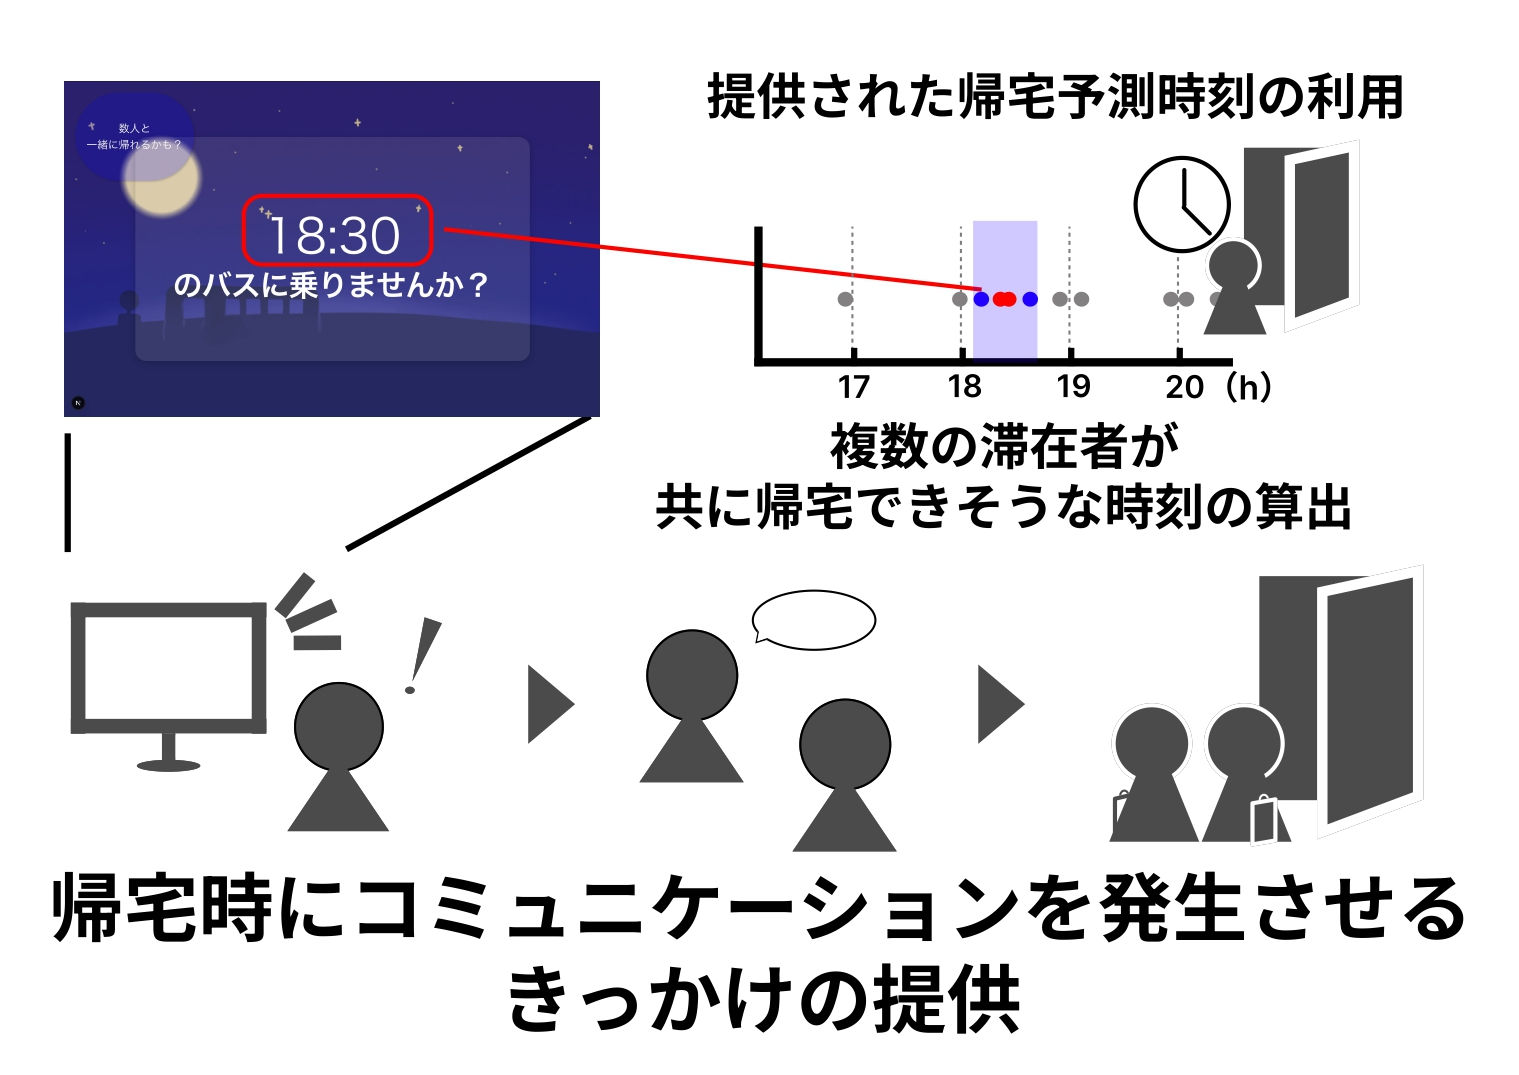
\includegraphics[width=75mm]{overview.jpg} % suzuki
    \caption{本研究の概要図}
    \label{fig:1}
    \vspace{-5mm}
\end{figure}

%--------------------------------------------
\section{leaving-match}
\label{sec:system}
% 一旦飛ばしてるなう
% システムフローを入れたい　バックエンドの話は時刻提示のところ
% 目指した設計の話はここか？ユーザへの強制力？能動的に動かさせるのを極力減らした話とか
% 名前の話どこに盛り込むんだ？　退出＋一致の単語の組み合わせ
本システムでは帰宅推奨時刻の算出，時刻の提示，組織内コミュニケーションツールを通じた投票の受付を主な機能とする．
コミュニティ内に行動を共にしたくない人がいる状況を許容する設計を目指した．

\subsection{システム構成}
本システムの構成は以下の通りである．
帰宅推奨時刻の算出が定期実行され，有効な場合のみデータベースに保存をする．
画面に提示する情報はデータベースに保存されたものを参照する．
Slackへのメッセージの送信は帰宅推奨時刻が近づいた判定がされた場合にのみWeb APIとして公開したエンドポイントを呼び出し実現している．
Slackから受信したメッセージはそのままデータベースに保存をし，表示側が投票締切時刻を過ぎた場合に集計をした．

\subsection{提示する時刻の算出}
% \subsubsection{帰宅予測時刻の取得}
先行研究で提案するシステム\cite{tex}が提供する帰宅予測時刻に基づき帰宅推奨時刻を算出する．
このシステムでは滞在履歴から来訪・帰宅時刻のみを取得し，GMMによるクラスタリングの結果得られた各成分の累積分布をデータ数で重み付けして合成し，一定の確率を超えた時刻を帰宅予測時刻としてWebAPIで提供している．
時間の経過に伴い滞在者の数や構成は変化するため，30分ごとに滞在者の帰宅予測時刻を取得し以下の手順で提示する時刻を算出する．

{\noindent\bf 最多区間の抽出}
%

滞在者の帰宅予測時刻が最多となる30分区間を抽出する．
これにより，多くの人が帰る時間帯を取得する．
% また，アプローチするメンバの選出も同時に行う．
%

{\noindent\bf 重み付き平均}
%

最多区間内で最も近い2点以上を取得し，平均値を基準とする．
全滞在者の時刻に平均値からの距離の逆数を重みとして付与し，積の和を求める．
重みの和で割ったものを帰宅推奨時刻としている．
%

{\noindent\bf バスの時刻と組み合わせた提示する時刻の取得}

%
帰宅推奨時刻に最も近いバスの時刻とその前後のバスの時刻を取得する．
選択肢を用意し，よりユーザの都合に合わせやすい設計にした．

\subsection{提示方法}
ディスプレイで3種類の画面表示と読み上げソフトで作成した音声での通知を行う．
1分ごとに画面を更新し，その時点のデータベースに保存された内容に応じて画面遷移させる．

\begin{figure}[htb]
    \centering
    \subcaptionbox{三択の時刻\label{fig:2a}}{% % suzuki
        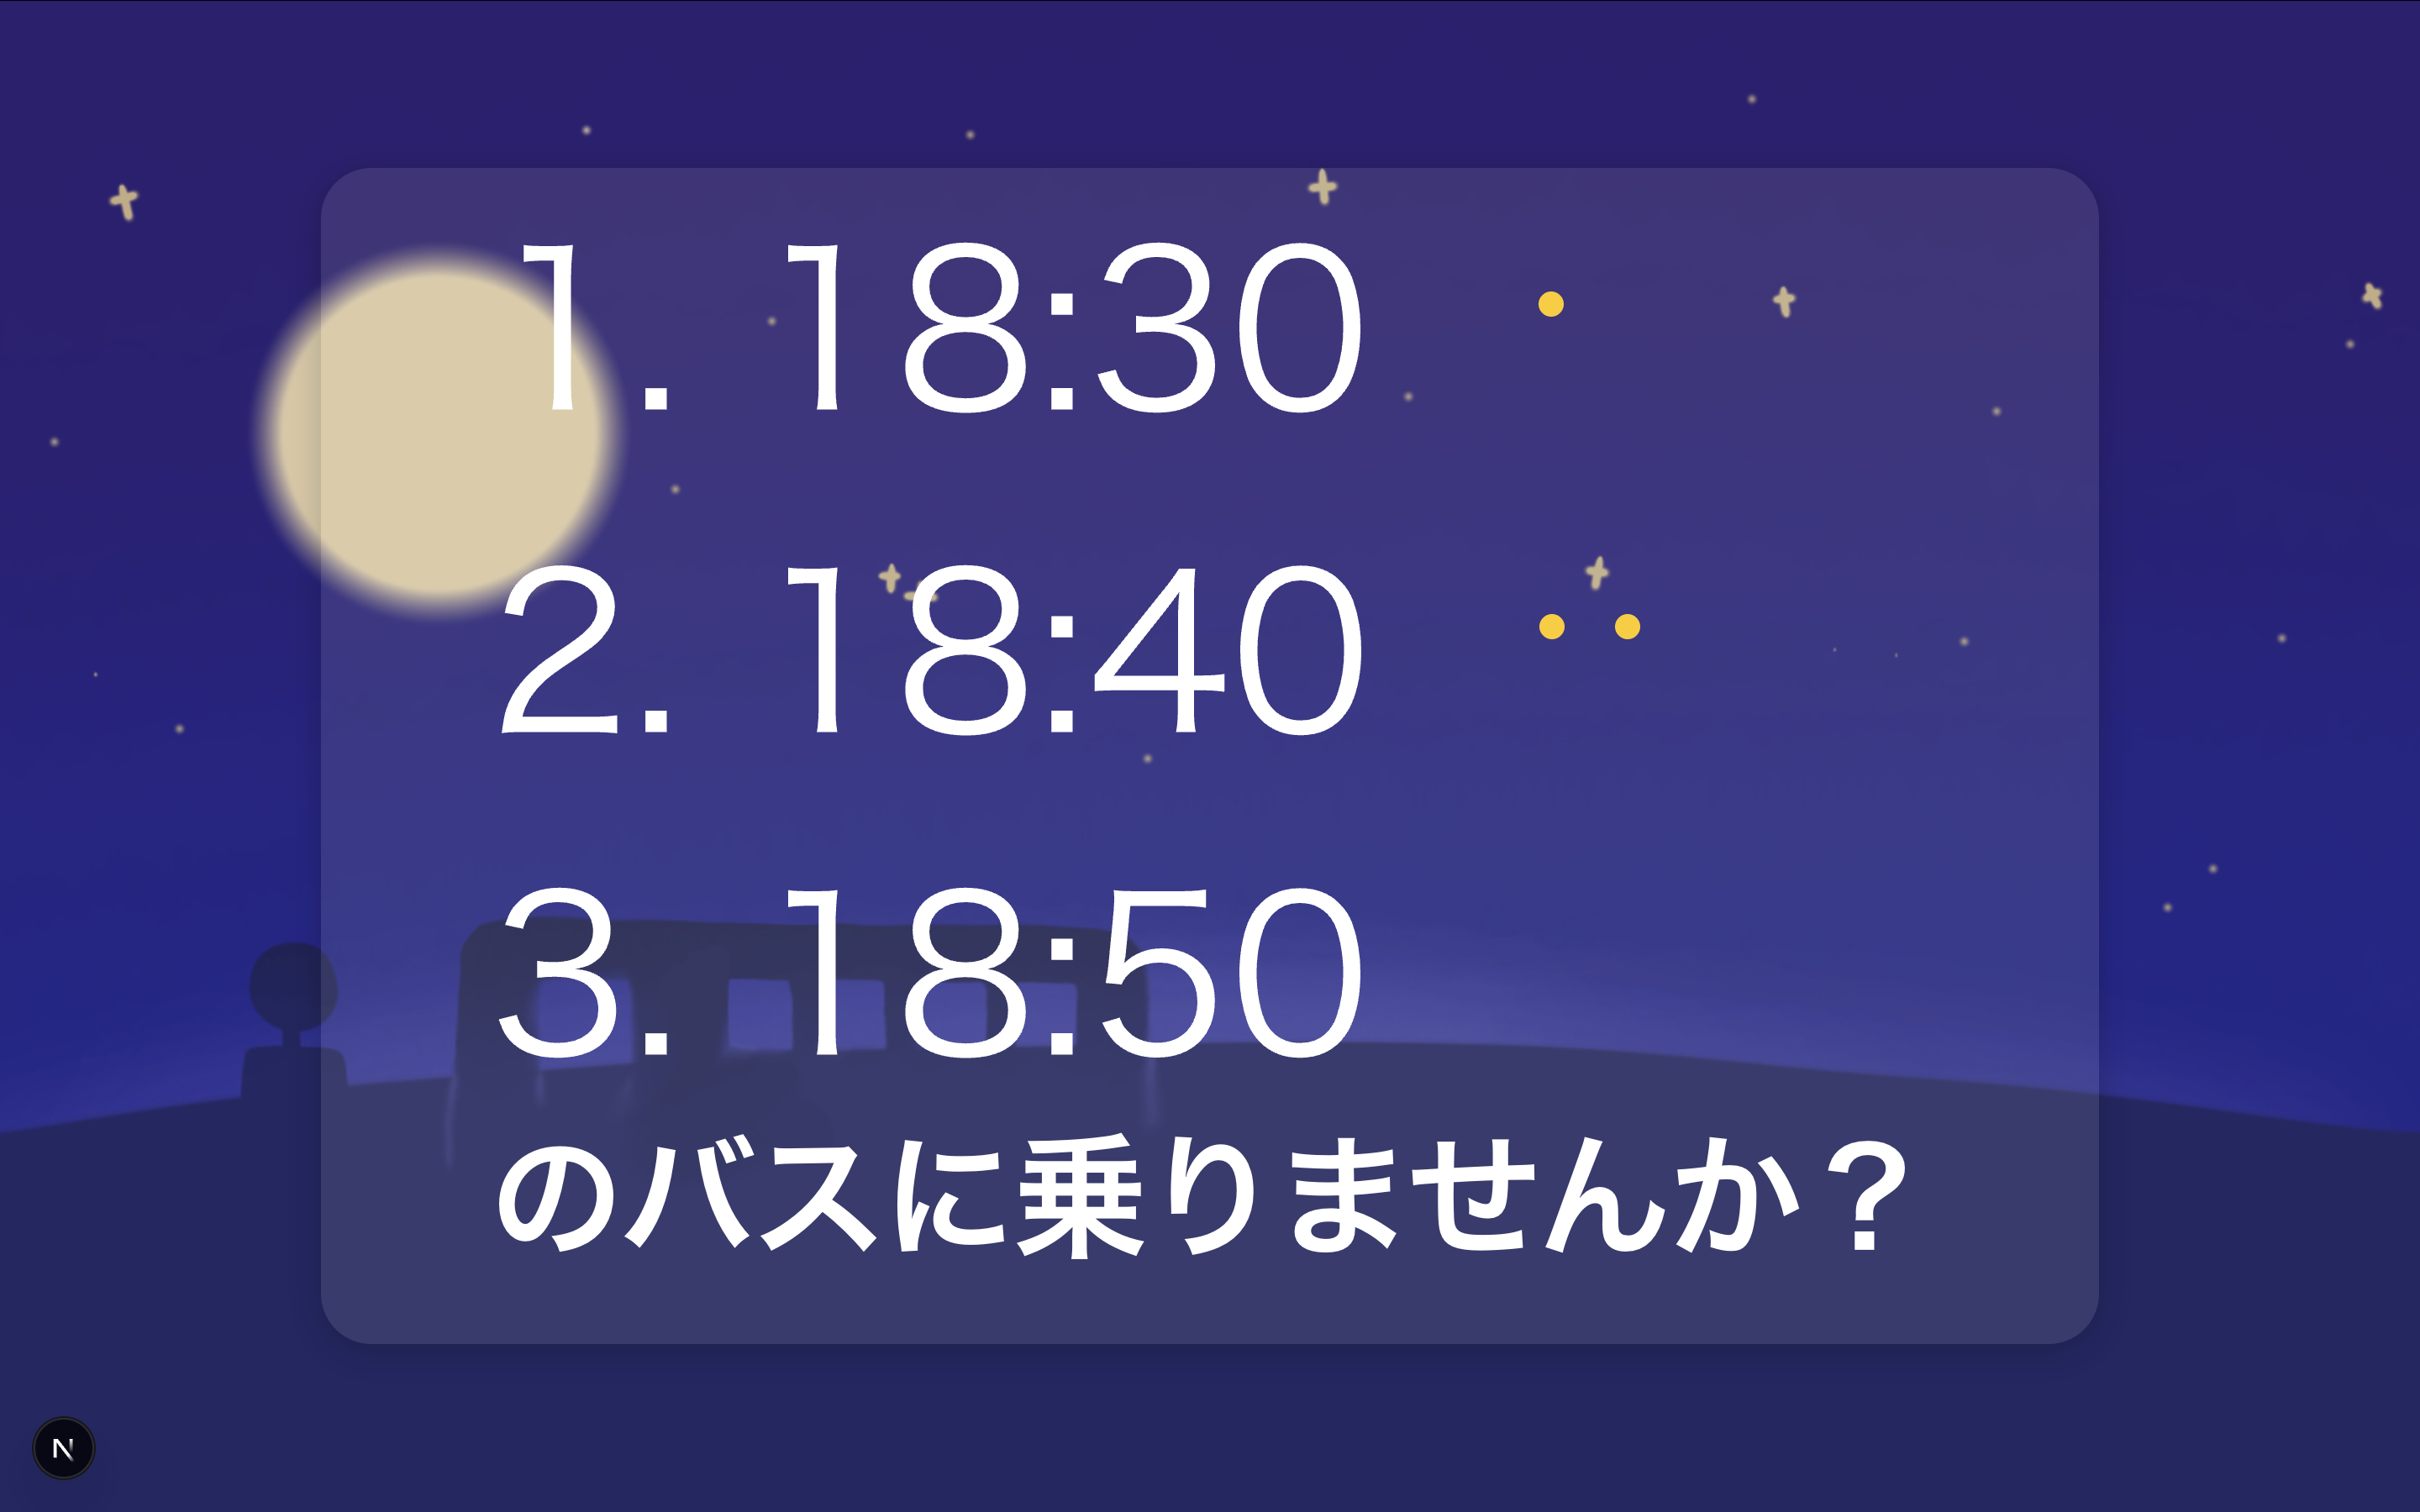
\includegraphics[height=24mm]{selectDisplay.png}}	% suzuki
    % \hspace{1mm}
    \subcaptionbox{最多投票の時刻\label{fig:2b}}{%	% suzuki
        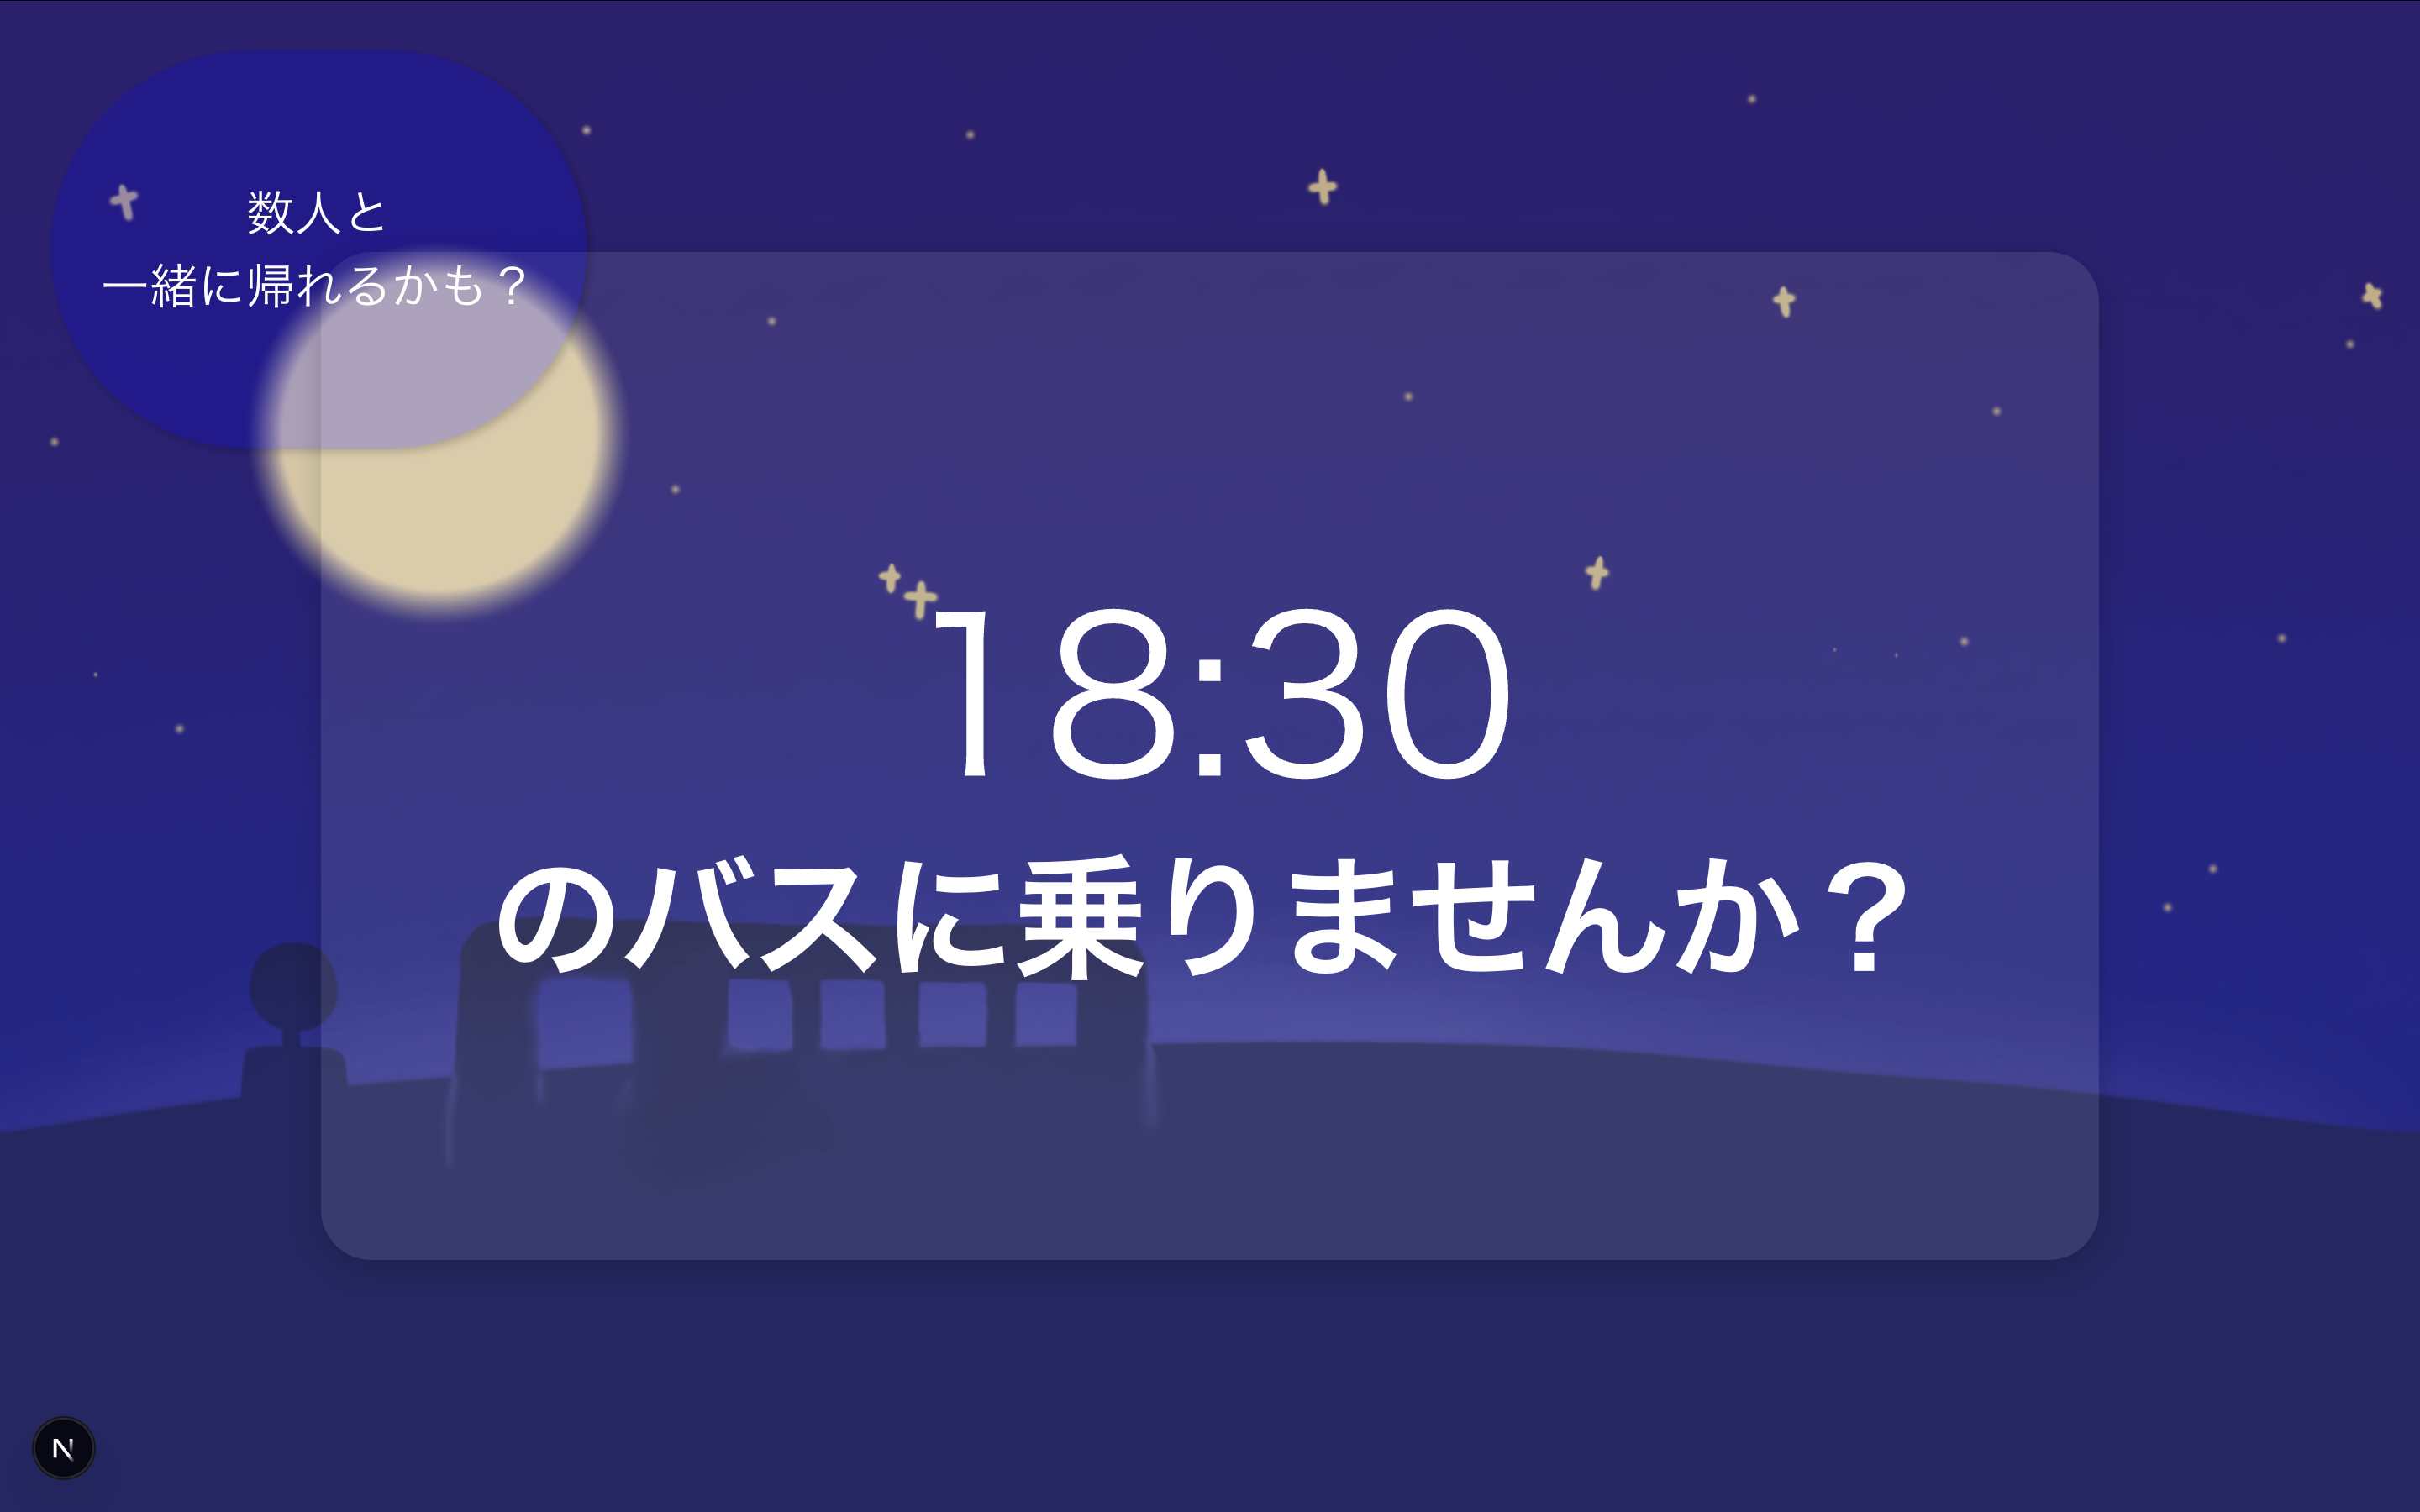
\includegraphics[height=24mm]{resultDisplay.png}}	% suzuki 
    \caption{時刻の提示を行う画面}
    \label{fig:2}
\end{figure}

{\noindent\bf 三択の時刻を提示する画面（図\ref{fig:2a}）}
%

この画面では三択の時刻と，それぞれの時刻への投票数を表示する．
この画面への遷移時に音声での通知も行い，画面表示の変化を認識させる．
また，投票状況を時刻横に反映し，他の人の投票を参考に帰宅時刻の検討や変更ができる設計とする．
現在時刻が投票締切時刻をすぎた際に最多投票の時刻を提示する画面へと自動的に遷移する．

{\noindent\bf 最多投票の時刻を提示する画面（図\ref{fig:2b}）}
%

この画面では投票数が最も多かった時刻とその投票数を表示する．
遷移時に投票数の集計をし，表示を行う．
投票がなかった場合は帰宅推奨時刻に最も近い時刻を，同票の時刻があった場合は早い時刻を表示し，より多くの人が帰る前の時刻を狙う．
また，投票数が少ない場合は「数人」のような抽象的な表現を，多い場合は具体的な数値を用いて投票数を表示し声かけを行うユーザの心理的負担を減らす設計とする．
現在時刻が表示している時刻をすぎた際に待機画面へと自動的に遷移する．

{\noindent\bf 待機画面}
%

以上の2つの画面でない状況を示す．
新たに三択の時刻が設定された際に三択の時刻を提示する画面へと自動的に遷移する．


\subsection{組織内コミュニケーションツールでの投票}
今回は研究室内で使用されているチャットツールであるSlackを採用し，SlackBotを用いてダイレクトメッセージ（以下DM）の送信と投票の受付を実現する．
%

帰宅推奨時刻の算出時に抽出した最多区間内のメンバに時刻情報を含んだDMを送信し投票を促す．
これによりユーザ側から近しい時刻に帰りそうな具体的なメンバを分からない状態にし，メンバ以外へのコミュニケーションの発生も狙う．
%

また，投票は1〜3の数字を入力させ打ち間違いを減らし，ユーザの手間を減らす．
複数の時刻への投票を可能とし，帰宅時刻を柔軟に変更できるユーザがより投票しやすい設計とする．

%--------------------------------------------
\section{評価実験}
\label{sec:description}
本システム稼働前の4週間と稼働させた4週間の2つの期間における滞在履歴の比較とアンケートの結果を用いて，このシステムの有効性を評価した．

\subsection{滞在履歴の比較}
我々の研究室で運用されている滞在推定システムと入り口付近のみを映したカメラを用いて，研究室に所属する大学生29名を対象に滞在履歴の比較を行った．
この29名は期間内に一度以上滞在履歴が残っており推定に利用するBLEビーコンの電池が切れていない確認が取れた人物を採用した．
研究室で使用頻度の高いテレビの横にモバイルディスプレイを設置し画面提示を行った．
複数人が共に退室した機会(以下同行機会)と退室同行機会における人数(以下同行人数)の二軸で評価した．


{\noindent\bf 同行機会の比較}
%

曜日ごとに1日あたりの同行機会の数を平均し，比較を行ったグラフが図\ref{fig:3a}である．
火曜日が多く日曜日が少ないなど曜日ごとの傾向を取得できたが，期間内での大きな変化は見られなかった．

{\noindent\bf 同行人数の比較}
%

曜日ごとに同行機会あたりの人数を平均し，比較を行ったグラフが図\ref{fig:3b}である．
2〜3人での同行が多いと分かったが，同様に期間内での大きな変化は見られなかった．

\begin{figure}[htb]
    \centering
    \subcaptionbox{平均同行機会\label{fig:3a}}{% % suzuki
        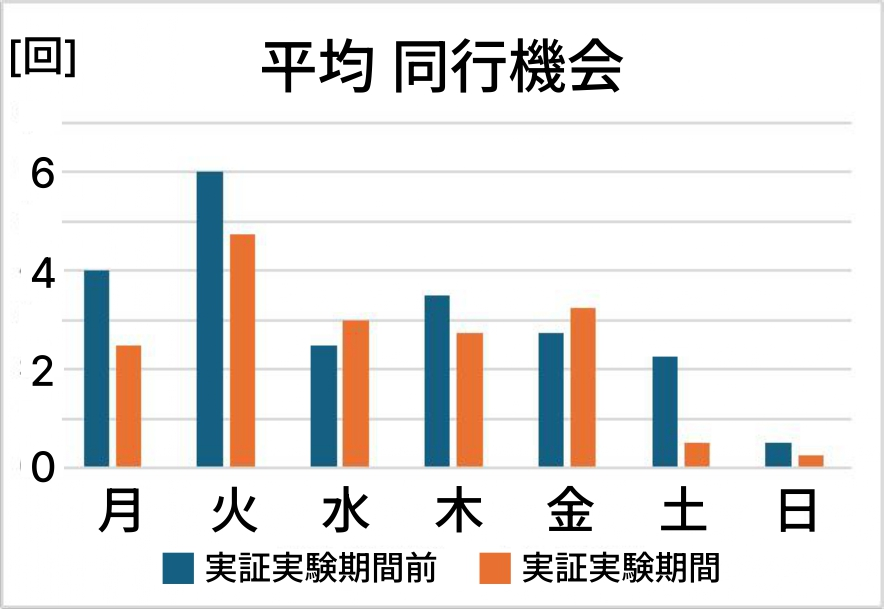
\includegraphics[height=29mm]{chance.jpg}}	% suzuki
    \subcaptionbox{平均同行人数\label{fig:3b}}{%	% suzuki
        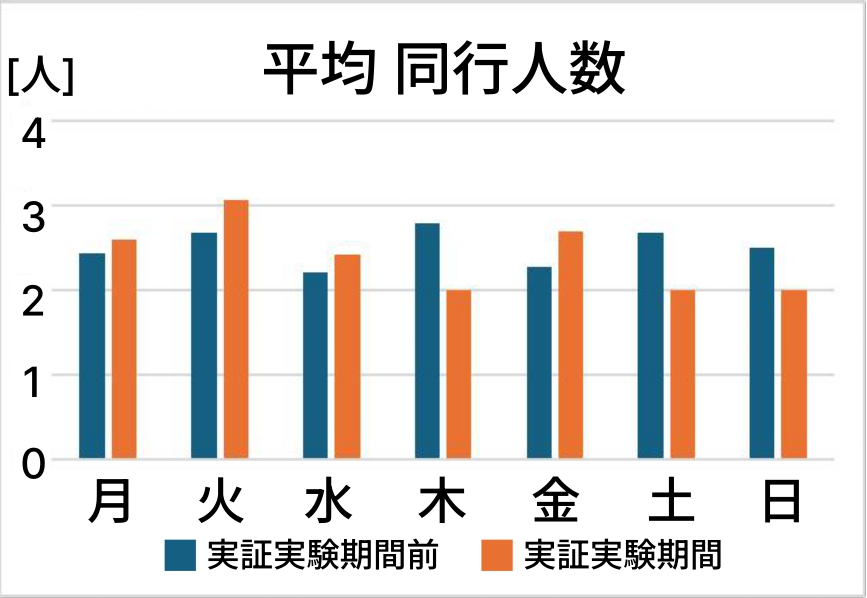
\includegraphics[height=29mm]{people.jpg}}	% suzuki 
    \caption{滞在履歴の比較グラフ}
    \label{fig:4}
\end{figure}

\subsection{アンケート結果}
実験対象である29名にアンケートを実施し，うち19名からシステムの利用率や退室時のコミュニケーションの有効性などについての回答を得た．

%

{\noindent\bf システムの利用率}
%

表示時刻に合わせて帰ったかという問いに対して，「ない」「月に一度のみ」「週に一回前後」「それ以上」という選択肢を用意し回答してもらったところ，月に一回以上利用したと答えた人は7人いた．
また，表示時刻を確認してコミュニケーションをとったかという問いに対してリッカート尺度を用いて1〜5で評価してもらったところ，4以上を選択した人は8人いた．
%

結果として19名のうち3割以上の人がこのシステムを活用し帰宅したと明らかになった．
%

{\noindent\bf 退室時のコミュニケーションの有効性}
%

期間内か否かに関わらず一緒に退室した際にコミュニケーションは生まれたかという問いに対して，「一人で退室することしかなかった」「一言二言だけ話した」「そのタイミングでのコミュニケーションで仲を深められた」という選択肢を用意し回答してもらった．
「そのタイミングでのコミュニケーションで仲を深められた」と答えた人が9人と最も多く，「一言二言だけ話した」と答えた人が6人とその次に多い．
これは退室時のコミュニケーションへの支援の妥当性を示している．



%--------------------------------------------
\section{今後の課題}
\label{sec:sammary}
今後の課題として主にアプローチ対象の拡張と実証実験期間の追加の2点が挙げられる．
本研究ではバスの時刻と組み合わせてアプローチを行ったため，他の公共交通機関を利用するユーザや，車などのより柔軟に帰宅時刻を変更できるユーザへのアプローチを検討する必要がある．
加えて，本研究では帰宅時のみに絞り支援を検討したが退室時全体を対象としたアプローチの検討も必要である．
さらに，システム稼働期間が4週間と短期間であったため一時的な変動の影響を受けやすく，安定的な変化を評価するには不十分であった．
したがって長期運用による評価が必要である．

%--------------------------------------------
% レジュメの節(section)構成は様々なものが考えられ，研究内容や制作内容によっても異なるが，一般的には研究背景，目的および研究概要を記述する「{\bf はじめに}」で始まる．
% そして研究全体のまとめ，結論，今後の課題を記述する「{\bf まとめ}」や「{\bf むすび}」で締めくくる．
% 全体的には5〜6個の節で構成され，必要に応じて小節(subsection)を用いる．

% \emph{研究の内容や記述する文章はオリジナルである必要がある．単に他の研究や実験を流用したり，インターネットや他の文献などの文章をそのままコピーして使用したりすることなどは決してあってはならない．レジュメは大量に印刷されて多くの人が読むため，コピーした文章の使用はすぐに誰かが見つける．} % changed to \emph by morimoto


%--------------------------------------------
% \section{図や表について}
% \label{sec:figure}

% 必要に応じて図や表を用いる．
% 使用した図や表についてはキャプションを付けるとともに，必ず本文中で図表番号を参照する．

% \emph{図や表は自分で作成したものを使用する．標準テストイメージ等を除き，インターネット等で入手した図や写真，表などをそのまま使ってはならない．} % changed to \emph by morimoto

% revised by morimoto
% レジュメは基本的にモノクロで印刷されるが，必要に応じてカラーの図や画像を用いることができる．
% またオフセット印刷で製本するため，十分に鮮明な図や画像を用意しておくとよい．

% revised by suzuki & morimoto (from EPS to PDF)
% \LaTeX の場合，図のファイルはPDF形式で用意することが推奨されている\cite{tex}．
% また，EPS形式を用いることができる．
% Illustratorなどのソフトで作成して，保存するときに\LaTeX で使用可能な画像形式を指定すればよい．
%
% PNG形式やJPEG形式を用いることもできるが，場合によっては図の外枠を明示的に指定する必要がある．

% 図 \ref{fig:1}は，単独の図である．
% また図 \ref{fig:2}は複数で構成される図である．
% またfigure*環境を用いることで1カラムの図を使用することも可能である．
%
% また，表のサンプルを表 \ref{tab:sample}に示す．

% \begin{figure}[htb]
%     \centering
%     % \includegraphics[width=40mm]{fig1.eps} % original
%     \includegraphics[width=40mm]{fig1.pdf} % suzuki
%     \caption{普通の図}
%     \label{fig:11}
% \end{figure}

% \begin{figure}[htb]
%     \centering
%     \subcaptionbox{多角形}{% % suzuki
%         \includegraphics[height=30mm]{fig2a.pdf}}	% suzuki
%     \hspace{3mm}
%     \subcaptionbox{楕円}{%	% suzuki
%         \includegraphics[height=30mm]{fig2b.pdf}}	% suzuki 
%     \caption{複数で構成される図}
%     \label{fig:2}
% \end{figure}

% \begin{table}[htb]
%     \centering
%     \caption{卒論卒制スケジュール}
%     \label{tab:sample}
%     \begin{tabular}{ll}\toprule
%         項目     & 締切日   \\ \midrule
%         レジュメ提出 & *月**日 \\
%         卒業論文提出 & *月**日 \\
%         発表会    & *月**日 \\ \bottomrule
%     \end{tabular}
% \end{table}

%--------------------------------------------
% \section{参考文献について}
% \label{sec:reference}

% 必要に応じて文末に参考文献を記述する．
% 記述した参考文献は必ず本文中で参照する．
% 参考文献の書き方と本文中での参照方法を確認すること \cite{ura, tex}．

%--------------------------------------------
% \section{PDFファイルの作成について}
% \label{sec:pdf}

% % revised by morimoto
% TexShop等でPDFを作成した場合，使用する図や画像によってはファイルサイズが非常に大きくなる場合がある．
% 例えば「Adobe Acrobat Pro」であれば，作成したPDFファイルを「別名で保存」から「最適化されたPDF」で保存し直すことで，ファイルサイズを小さくすることができる．
% 解像度は少なくとも300ppiは保つようにする．

% また，Mac付属のプレビューアプリでも，「書き出す」(「別名で保存」)で「Quartzフィルタ」の中の「Reduce File Size」を選択すればファイルサイズを小さくすることができる．
% ただし，デフォルト設定では出力されるPDFファイル中の画像の解像度が不足する可能性があるため，フィルタ設定を自作する必要があるかもしれない．ネットで検索すれば，Quartzフィルタの作成方法はすぐに見つかる．

%--------------------------------------------
% \section{まとめ}
% \label{sec:conclusion}

% レジュメは大量に印刷されて，同級生だけでなく後輩も見ることになる．それを踏まえて，しっかりした原稿を作成して欲しい．

%--------------------------------------------
% \begin{thebibliography}{9}
%     \bibitem{ura}
%     浦正広, 遠藤守, 山田雅之, 宮崎慎也, 岩崎公弥子, 毛利勝廣, 安田孝美, ``天文教育に向けたスマートフォンの活用による対話型の星座検索モデルの提案'', 情報文化学会誌, Vol. 19, No. 2, pp.42--49, 2012.

%     \bibitem{tex}
%     奥村晴彦, 黒木祐介, ``改訂第6版 \LaTeX2$\epsilon$ 美文書作成入門'', 技術評論社, 2013.

% \end{thebibliography}
% \end{document}

\begin{thebibliography}{9}
    \bibitem{ura}
    中野利彦ほか,
    ``Traveling Cafe:分散型オフィス環境におけるコミュニケーション促進支援システム'',
    インタラクション2006論文集,
    Vol.4,
    pp.227-228,
    2006.

    \bibitem{tex}
    林航平ほか,
    ``未来の在室状況予測と共通の話題に基づく来訪促進システムの提案'',
    DICOMO 2025 シンポジウム 論文集,
    pp.1552-1561,
    2025.

\end{thebibliography}
\end{document}

%%% Local Variables: 
%%% mode: japanese-latex
%%% TeX-master: t
%%% End: 
